\documentclass[twocolumn,showpacs,aps,pre]{revtex4-1}

% special 
\usepackage{ifthen}
\usepackage{ifpdf}
\usepackage{color}

\ifpdf
\usepackage{graphicx}
\usepackage{epstopdf}
\else
\usepackage{graphicx}
\usepackage{epsfig}
\fi
\graphicspath{{./Figs/}{./}}

% fonts
\usepackage{latexsym}
\usepackage{amsmath}
\usepackage{amstext}
\usepackage{amssymb}
\usepackage{bm}
\usepackage{wasysym}
\usepackage[pdftitle={},bookmarks]{hyperref}

% Standard symbols 
\newcommand{\sinc}{\mbox{sinc}}
\newcommand{\const}{\mbox{const}}
\newcommand{\trc}{\mbox{trace}}
\newcommand{\intt}{\int\!\!\!\!\int }
\newcommand{\ointt}{\int\!\!\!\!\int\!\!\!\!\!\circ\ }
\newcommand{\ar}{\mathsf r}
\newcommand{\im}{\mbox{Im}}
\newcommand{\re}{\mbox{Re}}

% Special symbols
\newcommand{\mass}{\mathsf{m}} 
\newcommand{\Mass}{\mathsf{M}} 

% Math constractions
\newcommand{\tbox}[1]{\mbox{\tiny #1}}
\newcommand{\bmsf}[1]{\bm{\mathsf{#1}}} 
\newcommand{\amatrix}[1]{\begin{matrix} #1 \end{matrix}} 
\newcommand{\eexp}[1]{\mathrm{e}^{#1}}
\newcommand{\pd}[2]{\frac{\partial #1}{\partial #2}}
\newcommand{\bra}[1]{\left\langle #1 \right|}
\newcommand{\ket}[1]{\left| #1 \right\rangle}
\newcommand{\braket}[1]{ \left\langle #1 \right\rangle}
\newcommand{\Braket}[2]{ \left\langle #1 \middle| #2 \right\rangle}
\newcommand{\BraKet}[3]{ \left\langle #1 \middle| #2 \middle| #3 \right\rangle}
\newcommand{\avg}[1]{\left\langle #1 \right\rangle}
\newcommand{\ola}{\protect\overleftarrow}
\newcommand{\ora}{\protect\overrightarrow}

% Equations
\newcommand{\be}[1]{\begin{eqnarray} \label{e#1}}
\newcommand{\beq}{\begin{eqnarray}}
\newcommand{\eeq}{\end{eqnarray}} 

% Text arrangement
\newcommand{\hide}[1]{}
\newcommand{\rmrk}[1]{\textcolor{red}{#1}}
%\newcommand{\Eq}[1]{\textcolor{blue}{Eq.\!\!~(\ref{#1})}} 
\newcommand{\Eq}[1]{{\textcolor{blue}{Eq.}}(\ref{#1})} 
%\newcommand{\Fig}[1]{\textcolor{blue}{Fig.}\!\!~\ref{#1}}
\newcommand{\Fig}[1] {{\textcolor{blue}{Fig.}}\ref{#1}}
\newcommand{\sect}[1]{{\bf #1.-- }}
\newcommand{\drawline}{\begin{picture}(500,1)\line(1,0){500}\end{picture}}
\newcommand{\bitem}{$\bullet$ \ \ \ }
\newcommand{\Cn}[1]{\begin{center} #1 \end{center}}
%\renewcommand{\cite}[1]{\textcolor{blue}{[\onlinecite{#1}}]} %{[\onlinecite{#1}]} 
\newcommand{\hrefl}[1]{\href{#1}{[link]}}

% temporary
%\renewcommand{\includegraphics}[2][]{\ \\ \ {\color{blue} FIGURE:} \ \\ \ }



%%%%%%%%%%%%%%%%%%%%%%%%%%%%%%%%%%%%%%%%%%%%%%%%%%%%%%%%%%%%%%%%%%%%%%%%%%%%%%%%%%%%%%%%%%%%%%%%%%%%%%%%%%%
\begin{document}

\title{Heat transport in low-dimensional random harmonic networks}

\author{Isaac Weinberg$^1$, Yaron de Leeuw$^1$, Tsampikos Kottos$^{2,3}$, Doron Cohen$^1$}
\affiliation{$^1$Ben-Gurion University of the Negev, Beer-Sheva 84105, Israel}
\affiliation{$^2$Department of Physics, Wesleyan University, Middletown, Connecticut 06459}
\affiliation{$^3$Department of Mathematics, Wesleyan University, Middletown, Connecticut 06459}

\begin{abstract}
We consider thermal transport in low-dimensional disordered harmonic networks of coupled masses. 
Utilizing known results regarding Anderson localization, we derive 
the actual dependence of the thermal conductance~$G$ on the length $L$ of the sample.  
This is required by nanotechnology implementations because for such networks 
Fourier's law ${G \propto 1/L^{\alpha}}$ with ${\alpha=1}$ is violated.  
%  
In particular we consider ``glassy" disorder in the coupling constants, 
and find an anomaly which is related by duality to the Lifshitz-tail regime
in the standard Anderson model. 
%
\end{abstract}

\pacs{76.50.+g,11.30.Er, 05.45.Xt}

\maketitle


%%%%%%%%%%%%%%%%%%%%%%%%%%%%%%%%%%%%%%%%%%%%%%%%%%%%%%%%%%%%%%
%%%%%%%%%%%%%%%%%%%%%%%%%%%%%%%%%%%%%%%%%%%%%%%%%%%%%%%%%%%%%%

The theory of phononic heat conduction in disordered low-dimensional networks is a central theme of research in recent years \cite{LLP03,
D08,LRWZHL12}. The interest in this theme is not only purely academic, but it is also motivated by the ongoing developments in nanotechnology.
In spite of the recent research efforts, the understanding of thermal transport is still at its infancy. This becomes more obvious if one compares 
with the achievements that have been experienced during the last fifty years in understanding and managing electron transport. In this respect 
even the microscopic laws that govern heat conduction in low dimensional systems have only recently start being scrutinized via both theoretical, 
numerical and experimental studies \cite{LLP03,D08,COGMZ08,NGPB09,LRWZHL12,ZL10,K1,K2}. These studies unveil many surprising results, the most 
dramatic of which is the violation of the naive expectation (Fourier's law) which states that the thermal conductance $G$ is inverse proportional 
to the size~$L$ of the system, namely, $G\propto 1/L^{\alpha}$ with ${\alpha=1}$. 

Currently it is well established that in low-dimensional disordered systems, in the absence of non-linearity, Fourier's law  is violated. The
underlying physics is related to the theory of Anderson localization of the vibrational modes \cite{D08,D01,LXXZL12,DL08,LD05,RD08,LZH01,
KCRDLS10a,KCRDLS10b}. On the basis of the prevailing theory \cite{D08,D01} it has been claimed that for samples with ``optimal" contacts ${\alpha=1/2}$, 
while in general $\alpha$ might be larger, say ${\alpha=3/2}$ for samples with ``fixed boundary conditions". Recently the ``optimal" value 
${\alpha=1/2}$ has been challenged by the numerical study of \cite{BZFK13}. These authors found a super-optimal value ${\alpha \sim 1/4}$ for 
moderate system sizes $L$, while asymptotically, in the presence of a pinning potential, $G$ decays exponentially as ${\exp(-\gamma L)}$. 


%%%%%%%

It is obvious that if the final goal 
is to achieve the control of heat flow on the nanoscale, 
first we have to understand the fundamental mechanisms of heat conduction, 
and provide an adequate description of its scaling with the system size for any~$L$, 
including the experimentally relevant cases of intermediate lengths.

In this paper, considering heat transport for low-dimensional disordered networks of coupled harmonic masses, we utilize known results from the field of mesoscopic electronic physics, in order to derive the actual $L$~dependence of $G$ for regular as well as for ``glassy" type of disorder. The information about the latter is encoded in the dependence of the inverse localization length $\gamma$ on the vibration frequency $\omega$. Our results explain the transition from optimal to super-optimal scaling behavior and eventually to exponential dependence on $L$. We address to the implications of the percolation threshold, and the geometrical bandwidth. Along the way we highlight a surprising anomaly that is related by duality to the Lifshitz-tail regime in the standard Anderson model, and test the borders of the one-parameter scaling hypothesis.  


%%%%%%%%%%%%%%%%%%%%%%%%%%%%
\sect{The model}
%
We consider a one-dimensional network of $L$ harmonic oscillators of equal masses. 
The system is described by the Hamiltonian 
% 
\begin{equation}
{\cal H} = {1\over 2} P^T P + {1\over 2} Q^T \bm{W} Q 
\label{Hmatrix} 
\end{equation}
%
where $Q^T\equiv(q_1,q_2,\cdots,q_N)$, and $P^T\equiv(p_1,p_2,\cdots,p_N)$ 
are the displacement coordinates and the conjugate momenta. 
The real symmetric matrix  $\bm{W}$ is determined by the spring constants.
Its off-diagonal elements $W_{nm}{=}-w_{nm}$ originate from 
the coupling potential $(1/2)\sum_{m,n}w_{nm}(q_n-q_m)^2$, 
while its diagonal elements contain an additional 
optional term that originate from a pinning potential ${(1/2)\sum_n v_n q_n^2}$ 
that couples the masses to the substrate. 
Accordingly ${W_{nn}=v_n+\sum_m w_{nm}}$. 
For a chain with near-neighbor transitions we use 
the simplified notation ${w_{n{+}1,n} \equiv w_n}$.  


In general the interest is in quasi one-dimensional networks, 
for which $\bm{W}$ is a banded matrix with ${1{+}2b}$ diagonals. 
The heat conduction of such networks has been investigated numerically 
in \cite{BZFK13}, with puzzling findings that have not been explained 
theoretically. We shall see that the essential physics can be 
reduced to single channel ($b=1$) analysis. On top we would like  
to consider not only weakly disordered network, but also 
the implications of ``glassy" disorder as defined below.   


%%%%%%%%%%%%%%%%%%%%%%%%%%%%%%%%%%%%%%%%%%%%%%%%%%%%%%%%%%
\sect{The disorder}
%
Both the $w_{nm}$ and the $v_n$ are assumed to 
be random variables. The diagonal-disorder due to the pinning
potential is formally like that of the standard Anderson model 
with some variance ${\mbox{Var}(v)=\sigma_{\parallel}^2}$.    
The off-diagonal disorder of the couplings might be 
weak with some variance ${\mbox{Var}(w) \equiv \sigma_{\perp}^2}$, 
but more generally it can reflect the glassiness of the network. 
%
By ``glassy disorder" we mean that the coupling~$w$ has an 
exponential sensitivity to physical parameters.  
For ``random barrier" statistics ${ w \propto \eexp{-B} }$, 
where $B$ is uniformly distributed within $[0,\sigma]$. 
For ``random distances" statistics ${ w \propto \eexp{-R} }$,
where $R$ is implied by Poisson statistics. 
The probability distribution in the latter case is 
%
\beq
P(w) \ \ = \ \ \frac{s}{w_c^{s}} w^{s-1} \ (w<w_c)
\eeq
%
where~$s$ is the normalized density of the sites.
Large $s$ is like regular weak disorder, while small $s$ 
implies glassy disorder that features log-wide distribution  
(couplings distributed over several orders of magnitude). 
The case $s=0$ with an added lower cutoff 
formally corresponds to ``random barriers". 


%%%%%%%%%%%%%%%%%%%%%%%%%%%%%%%%%%%%%%%%%%%%%%%%%%%%%%%%%%
\sect{Resistor-network perspective}
%
It is useful to notice that the problem of phononic heat conduction 
in the absence of a pinning potential is formally equivalent 
to the analysis of a rate equation, where the spring-constants 
are interpreted as the rates~$w_{nm}$ 
for transitions between sites~$n$ and~$m$. 
Optionally it can be regarded as a resistor-network problem 
where $w_{nm}$ represent connectors. 
%
We define $w_0$ as the average hopping rate between sites. 
We later justify that it is formally the same 
as the {\em conductivity} of the corresponnding resistor-network.   
For a ${b=1}$ chain the ``serial addition" rule 
implies that it equals the harmonic average ${w_0=[(s{-}1)/s]w_c}$. 
For ${s<1}$ the network is no longer percolating ${w_0=0}$.  
In the present context $w_0$ determines the speed of sound (see below).


% PN, banded 
%%%%%%%%%%%%%%%%%%%%%%%%%
\begin{figure}
\centering
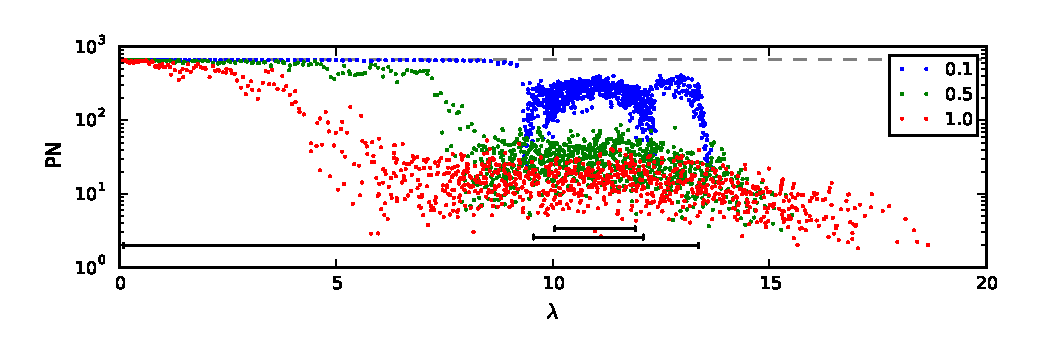
\includegraphics[width=\hsize]{pthBanded}
 
\caption{The participation number (PN) \cite{rmrkA} of the eigenstates of a conservative banded matrix 
are plotted against their eigenvalues $\lambda$.
The $0< |m-n| \le b$ elements of $\bm{W}$ are random numbers $w\in[1-\varsigma,1+\varsigma]$ (box distribution).
The values of $\sigma$ are indicated in the legend  
(note that the numerics of \cite{BZFK13} corresponds to $\varsigma{=}0.5$). 
The number of bands is $b{=}5$, and the length of the sample is $N{=}1000$ with periodic boundary conditions. 
The support of the clean-ring channels is indicted by the lower horizontal lines.
We observe the gradual blurring of the non-disordered band structure. 
All the eigenstates that have large PN reside in the lower part of the spectrum and belong to a single channel. 
}

\label{f1}
\end{figure}



%%%%%%%%%%%%%%%%%%%%%%%%%%%%%%%%%%%%%%%%%%%%%%%%%%%%%%%%%%
\sect{The spectrum}
%
The eigenvalues $\lambda_k$ are determined via diagonalization $\bm{W}Q=\lambda Q$, 
from which one deduces the eigen-frequencies via ${\lambda_k=\omega_k^2}$.
In the absence of disorder the eigenmodes are Bloch states with 
%
\beq
\lambda_k \ = \ 2w_0 \sum_{r=1}^{b}[1-\cos(r k)] \ \ \equiv \ \ \omega_k^2
\eeq  
%
where~$k$ is the associated wavenumber. 
For a single channel $\lambda=2w_0(1{-}\cos k) \approx w_0 k^2$, 
where the small-$k$ approximation holds close to the band floor.
%
With disordered couplings, but in the absence of a pinning potential 
the lowest eigenvalue is still $\lambda_0=0$,  
which corresponds to the trivial extended state ${Q=(1,1,...,1)}^T$, 
that is interpreted as the ergodic state in the context of rate equations. 
%
All higher eigenstates are exponentially localized, and are characterized 
by a spectral density $\varrho(\omega)$. 


In \Fig{f1} we provide a numerical example considering a quasi-one dimensional 
sample with ${b=5}$ channels.  
%
It is important to observe that at the bottom of the band 
a single channel approximation is most appropriate.
%
Hence within the framework of the Debye approximation 
the dispersion is $\omega \approx c k$, with ${c=\sqrt{w_0}}$. 
For $b{\gg1}$ it is easily found that $c\mapsto[(1/3)b^3]^{1/2}c$.
Either way the low-frequency spectral density 
is $\rho(\omega) \approx L/(\pi c)$.  
%
Weak disorder does not affect much this result. 
Using the resistor-network interpenetration 
one identifies $w_0$ as the conductivity (see previous paragraph). 
It is finite provided the network is percolating.  


%%%%%%%%%%%%%%%%%%%%%%%%%%%%%%%%%%%%%%%%%%%%%%%%%%%%%%%%%%
\sect{Localization}
%
The disorder significantly affects the eigenmodes: rather than being extended 
as assumed by Debye, they become exponentially localized. 
We use the standard notation $\gamma(\omega)$ for the inverse localization length: 
%
\beq
\label{locdef}
\gamma(\omega) \ \ = \ \ -\lim_{L\rightarrow \infty}{1\over 2}{\langle \ln(g) \rangle_{\omega} \over L}
\eeq
%
where $\langle\cdots\rangle$ indicates an averaging over disorder realizations, 
and~$g$ is the transmission. The notion of transmission is physically appealing here,  
because we can regard~$\bm{W}$ as the Hamiltonian of an electron in a tight binding model. 
The transmission can be calculated from the transfer matrix $\bm{T}$ of the sample:
%
\beq
\label{gTMM}
g \ \ = \ \ \frac{4|\sin(k)|^2}{|T_{21}-T_{12}+T_{22}\exp(ik)-T_{11}\exp(-ik)|^2}
\eeq
%
where for a single channel ($b=1$) network
%
\be{5}
\bm{T} \ \ = \ \ \prod_{n=1}^{n=L} 
\left(\amatrix{
\frac{\lambda-(v_n + w_{n}+w_{n+1})}{w_{n+1}} & -\frac{w_{n}}{w_{n+1}} \cr 1 & 0 
}\right)
\eeq
%
Above it is assumed that the sample is attached to two non-disordered leads.
Optimal coupling requires the hopping-rates there to be all equal 
to the ``conductivity"~$w_0$, meaning same speed of sound. This observation 
has been verified numerically (not displayed). 

%%%%%%%%%%%%%%%%%%%%%%%%%%%%%%%%%%%%%%%%%%%%%%%%%%%%%%%%%%
\sect{Born approximation}
%
In the absence of disorder $\bm{W}$ describes hopping 
with some rate $w_0$, and the eigenstates are free waves labeled by~$k$. 
With disorder the~$w_0$ of the unperturbed Hamiltonian is 
loosely defined as the average~$w$. Later we shall go beyond 
the Born approximation and will show that it should 
be the harmonic average (as already defined previously).   
%
The disorder couples states that have different~$k$. 
For diagonal disorder ("pinning") the couplings are proportional to the 
variance of the diagonal elements, 
namely ${ \overline{|W_{k,k'}|^2} = (1/L)\text{Var}(v)}$.
%
For off-diagonal disorder (random spring constants) 
the  couplings are proportional to the variance  of 
the off-diagonal elements, and depends on~$b$ and on~$k$ too:
%
\beq
\overline{\left|W_{k',k}\right|^2}  =  \frac{\text{Var}(w)}{L} \ \sum_{r=1}^{b} \left[2\sin(rk'/2) \, 2\sin(rk/2)\right]^2 
\eeq
%
It follow that for small~$k$ we have ${|W_{k,k'}|^2 \propto b^5 \sigma_{\perp}^2 k^4}$. 


The Fermi-Golden-Rule (FGR) picture implies that 
the scattering rate is ${\tau^{-1}= 2\pi \varrho(\omega) \overline{\left|W_{k',k}\right|^2}}$. 
%
The Born approximation for the mean free path is ${\ell=[d\lambda/dk]\tau}$, 
where the expression in the square brackets is the group velocity 
in the electronic sense ($\lambda$ is like energy). 
The Debye approximation implies $d\lambda/dk \approx 2[c^2]k$.
% 
The inverse localization length is $\gamma=(2\ell)^{-1}$. 
From here (without taking the small $k$ approximation) it follows that 
%
\beq \label{FGRv}
\gamma(\omega) \ \ &\approx& \ \ 
\frac{1}{8}\left[\frac{9}{b^6}\right]\left(\frac{\sigma_{\parallel}}{w_0}\right)^2  \left(\frac{1}{\sin(k)}\right)^2
\\ \label{FGRw} &+& \ \ 
\frac{1}{8}\left[\frac{9}{5b}\right]\left(\frac{\sigma_{\perp}}{w_0}\right)^2  \left( 2\tan\left(\frac{k}{2}\right) \right)^2
\eeq
%
where the prefactors in the square brackets assume ${b\gg1}$, and should be replaced by unity for ${b=1}$.
In the absence of pinning the localization length diverges ($\gamma \propto k^2$) 
at the band floor, as assumed by Debye. This behavior is demonstrated in \Fig{f2} 
for two types of glassy disorder. The deviations from \Eq{FGRw} 
will be explained in the next paragraphs. 




% gamma vs $k$, box disorder
%%%%%%%%%%%%%%%%%%%%%%%%%
\begin{figure}

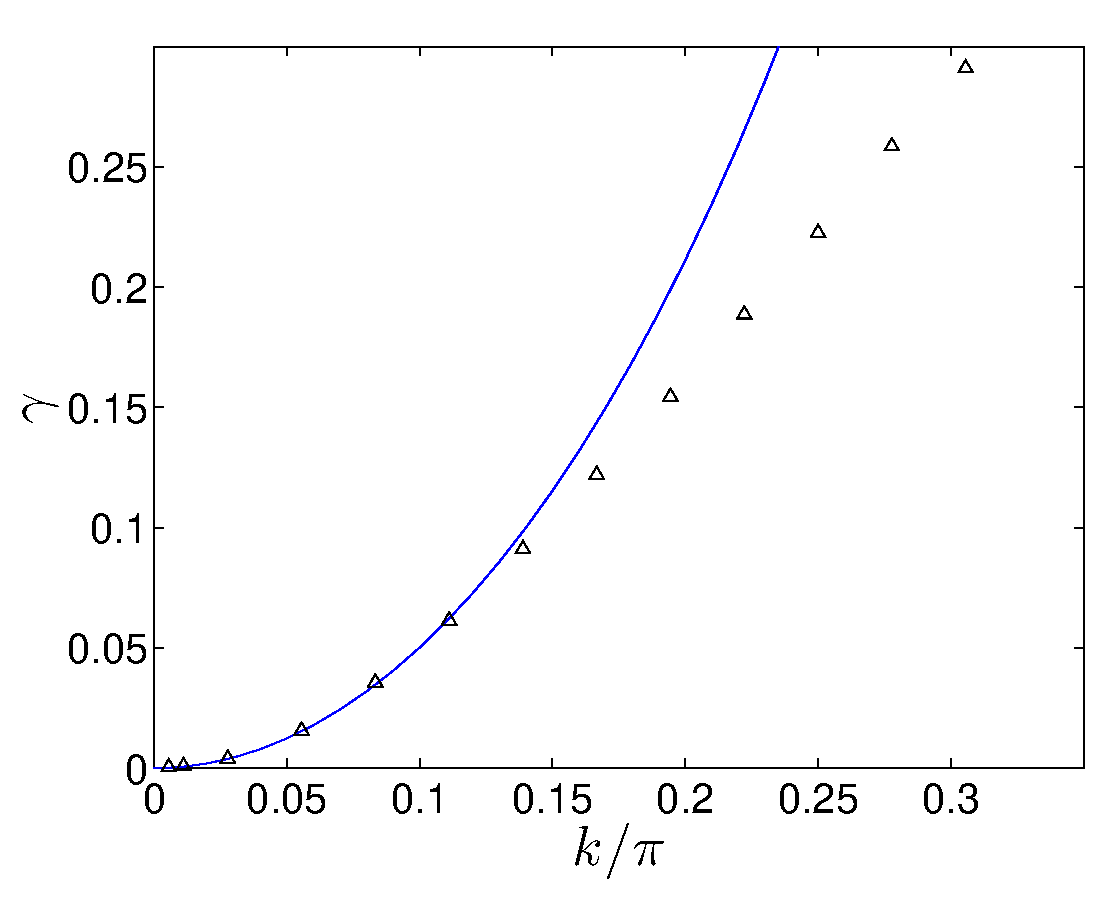
\includegraphics[width=4cm]{gammaVSkBX}
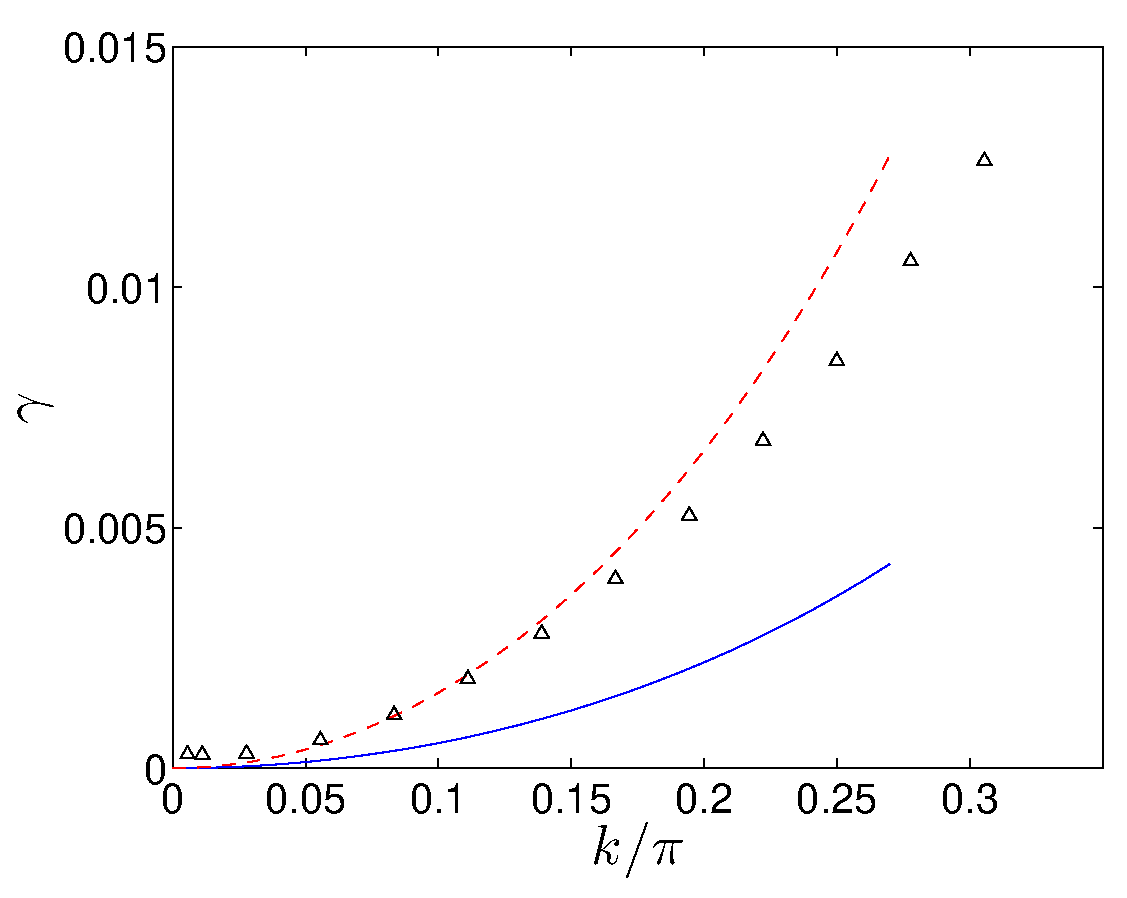
\includegraphics[width=4cm]{gammaVSkPL}

%\includegraphics[width=7cm]{gamma_k_logbox10}
%\includegraphics[width=7cm]{gamma_k_power_s_3}

% old plots for logbox disorder with sigma=10,35, and for powerlaw disorder
%\includegraphics[width=0.4\textwidth]{gamma10}
%\includegraphics[width=0.4\textwidth]{gamma35}
%\includegraphics[clip,width=10cm]{gamma_alpha.png}

\caption{The inverse localization length $\gamma$ versus $k$ 
for logbox distributed rates with $\sigma=10$ (a);   
and for powerlaw distributed rated with $s=4$ (b).  
Pure off-diagonal disorder is assumed.
The numerical results here and in the next figure 
are based on the transfer matrix method (symbols), 
with several hundreds of realizations up to ${L\sim10^4}$.
They are compared to the naive Born expectation \Eq{FGRw} (solid blue line).
In panel (b) the upper dashed red line is based on our improved 
estimate for ``glassy disorder"  \Eq{e12}, 
while in (a) it coincides with the naive estimate (hence not indicated). 
The inverse localization length $\gamma$ is over-estimated 
as $k$ becomes larger due to the Lifshitz tail anomaly (see text).  
}
\label{f2}
\end{figure}





%%%%%%%%%%%%%%%%%%%%%%%%%%%%%%%%%%%%%%%%%%%%%%%%%%%%%%%%%%
\sect{Beyond Born}
%
The Born approximation has assumed weak disorder. 
Here we would like to consider the more general case 
of glassy disorder. For this purpose we write 
the equation ${\bm{W}\psi = \lambda \psi}$ for the eigenstates 
as a map of a single variable ${r_n=\psi_{n}/\psi_{n-1}}$,   
namely  ${r_{n+1} = -R_n/r_n - A_n}$,  
where ${R_n=w_{n-1}/w_{n}}$, and ${A_n = (\lambda-v_n-w_n-w_{n-1})/w_n}$.
In the case of diagonal disorder it takes the from  
%
\be{8}
r_{n+1} \ = \ -\frac{1}{r_n} - \epsilon + f_n
\eeq
%
where $f_n=v_n/w_0$ is the scaled disorder 
and $\epsilon=(\lambda/w_0){-}2 \equiv 2\cos(k)$ 
is the scaled energy 
measured from the center of the band.
%
Without the random term $f_n$ this map has a fixed-point 
that is determined by the equation ${ r^2+\epsilon r +1=0 }$, 
with elliptic solution for ${\epsilon\in[-2,2]}$. 
The random term is responsible for having 
a non zero inverse localization length.
The Born approximation \Eq{FGRv} is written as  
%
\be{9}
\gamma \ \ = \ \ -\langle \ln(r) \rangle \ \ \approx \ \ \frac{1}{8} \, \frac{ \mbox{Var}(f)}{\left[1-(\epsilon/2)^2\right]}
\eeq
% 
This standard estimate does not hold close to the band-edge $\epsilon_0{=}{-}2$. 
The energy scale that controls the so-called Lifshitz tail region 
is $\epsilon_c = [\mbox{Var}(f)]^{2/3}$.
In the region $|\epsilon-\epsilon_0|<\epsilon_c$ the inverse localization 
length has finite value $\gamma \sim \sqrt{\epsilon_c}$.
This observation has no dramatic consequences at this stage 
since we assume a weak pinning potential. 


%%%%%%%%%%%%%%%%%%%%%%%%%%%%%%%%%%%%%%%%%%%%%%%%%%%%%%%%%%
\sect{Duality}
%
We now turn to consider the glassy disorder due to the dispersion of the $w_n$. 
Here we cannot trust the Born approximation because a small parameter is absent. 
However, without any approximation we can write the map in the form 
%
\be{10}
r_{n+1} \ \ = \ \ R_n \left( 1 - \frac{1}{r_n}\right) + 1 -\frac{\lambda}{w_n} 
\eeq
%
For $\lambda{=}0$ the zero momentum state is a solution as expected, 
irrespective of the disorder: the randomness in $R_n$ is not effective 
in destroying the ${r=1}$ fixed point. Therefore, for small $\lambda$, 
we can set without much error ${R_n=1}$. The formal argument that justifies 
this approximation is based on the linearization ${(r_{n+1}-1)=R_n(r_n-1)}$, 
and the observation that the product ${R_1R_2R_3...}$ remains of order unity. 
On the basis of this insight \Eq{e10} reduces to \Eq{e8} with the identifications 
%
\beq
\epsilon = -2 + \frac{\lambda}{w_0}, 
\ \ \ \ \ f_n = -\lambda \left(\frac{1}{w_n}-\frac{1}{w_0} \right)
\eeq 
%
The expression for~$\epsilon$ justifies the identification of the harmonic average $w_0$ 
as the effective coupling. Furthermore, we observe that there is an {\em emergent} small parameter, 
namely, the dispersion of~$f$, which is proportional to $\lambda$ irrespective of the glassiness. 
Thus we have deduced a {\em duality} between ``strong" glassy disorder and ``weak" diagonal disorder.
%
In the context of the dual problem we can use with confidence the Born approximation \Eq{e9}, leading to  
%
\be{12}
\gamma \ \ \approx \ \ \frac{1}{8} w_0^2 \, \mbox{Var}\left(\frac{1}{w}\right)  
\, \frac{4\left(\frac{\lambda}{2w_0}\right)}{2-\left(\frac{\lambda}{2w_0}\right)}
\eeq
% 
This would coincide with the primitive Born approximation \Eq{FGRw} 
if we could replace the harmonic averages by algebraic averages, namely,  
%
\beq
\frac{\mbox{Var}(1/w)}{\langle 1/w \rangle^2} 
\ \ \mapsto \ \ 
\frac{\mbox{Var}(w)}{\langle w \rangle^2} 
\eeq 
%
For log-box distribution the two types of averages provide exactly the same result, but for 
power-law disorder the two prescriptions differ enormously. This is demonstrate in \Fig{f2}, 
were we present our numerical results together with the theoretical predictions. 
%
Irrespective of that, the inverse localization length $\gamma$ is over-estimated as $k$ becomes larger. 
We can trace the origin of this discrepancy to the Lifshitz anomaly in the Anderson model.
The condition ${|\epsilon-\epsilon_0|<\epsilon_c}$ translates into ${\lambda > w_0^{-3}[\mbox{Var}(1/w)]^{-2}}$.
Thus the anomaly develops not at the band floor but as we go up in~$\omega$, 
where the inverse localization length becomes $\gamma \propto \omega^{4/3}$ 
instead of $\gamma \propto \omega^2$. 



% var[ln(g)] and ln<g> vs <ln(g)>
%%%%%%%%%%%%%%%%%%%%%%%%%%%%%%%%%%%%%%%%%%%

\begin{figure}

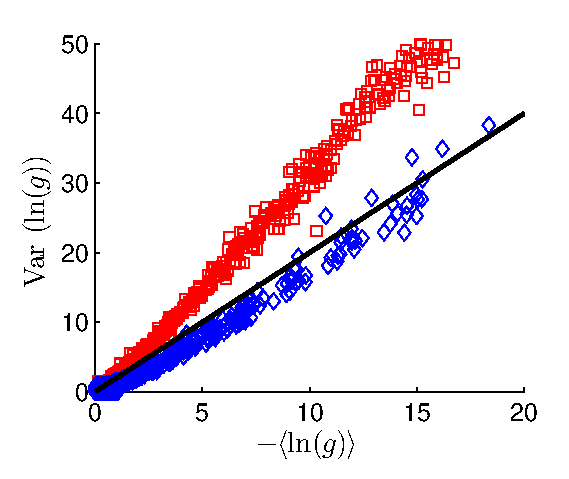
\includegraphics[clip,width=4cm]{varVSavg}
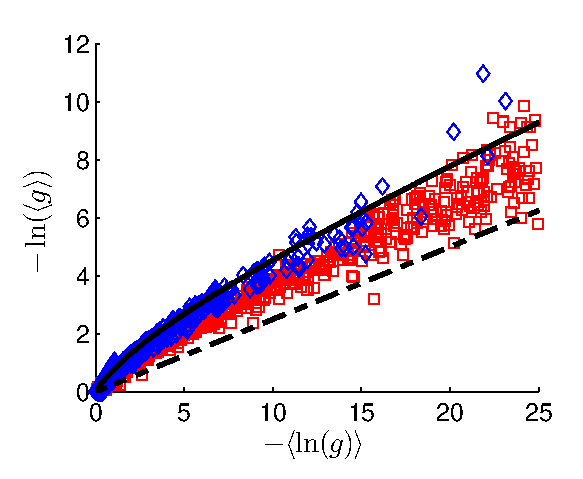
\includegraphics[clip,width=4cm]{avgVSavg}

%\includegraphics[clip,width=6cm]{var_lng_lng}
%\includegraphics[clip,width=6cm]{lng_lng}

%old plots for logbox disorder with sigma=10,35
%\includegraphics[width=5.5cm]{varlng_lng_dis10}
%\includegraphics[width=5.5cm]{varlng_lng_dis35}

\caption{ \footnotesize 
Testing one parameter scaling for glassy disorder. 
The variance of $\ln(g)$ (left panel) and the log of the average $-\ln\langle g \rangle$ (right panel)
are plotted against the scaling parameter $-\langle \ln(g) \rangle$. 
The calculation is done for powerlaw distributed rates 
with ${s=15}$ (blue diamonds) and ${s=1.2}$ (red squares).
The solid line is the standard one parameter scaling prediction for weak disorder, 
and the dashed line is its asymptotic approximation. 
One observes that an anomaly develops as the disorder becomes glassy.}

\label{f3}
\end{figure}



%%%%%%%%%%%%%%%%%%%%%%%%%%%%%%%%%%%%%%%%%%%%%%%%%%%%%%%%%%
\sect{The average transmission}
%
For the calculation of the heat transport we have to know 
what is  ${ g(\omega) \equiv \langle g \rangle_{\omega} }$. 
Given $\gamma$ the common approximation 
is ${ \langle g \rangle \approx \eexp{-(1/2)\gamma L}}$.
But in-fact this asymptotic approximation can be trusted 
only for very long samples. More generally, assuming weak disorder, 
the following result can be derived~\cite{Abrikosov,Shapiro,Izrailev}:
%
\be{14}
\langle g \rangle \ = \ 
\int_0^\infty\mathrm{d} u
\ \frac{2\pi u\tanh(\pi u)}{\cosh(\pi u)}
\ \mathrm{e}^{-\left[\left(\frac{1}{4}+u^2\right)\gamma L\right]}
\label{gabrik}
\eeq
%
The question arises whether this relation can be trusted 
also in the case of a glassy disorder, where the 
one-parameter scaling assumption cannot be justified.
%
This is tested in \Fig{f3}. For weak disorder (large $s$) 
the expected relation between the first and second moments 
of $x=-\ln(g)$ is confirmed, namely ${\text{Var}(x)=2\langle x \rangle}$.
For strong glassy disorder (small $s$) clear deviation 
from this relation is observed. 

Still we see in \Fig{f3}b that the failure of one-parameter scaling 
is not alarming for $\langle g \rangle = \langle \exp[-x] \rangle$.
The exact calculation of the integral is the solid line,
while the asymptotic result $\exp[-(1/2)\langle x \rangle]$ 
is indicated by dashed line. Note that the latter 
implies ${\langle g \rangle = \exp[(1/4)\langle\ln(g)\rangle]}$. 
We realize that the asymptotic approximation might be poor, 
but the exact calculation using \Eq{e14} is quite satisfactory. 


% G
%%%%%%%%%%%%%%%%%%%%%%%%%%%%%%%%%%%%%%%%%%%%%%%%%%%%%
\begin{figure}

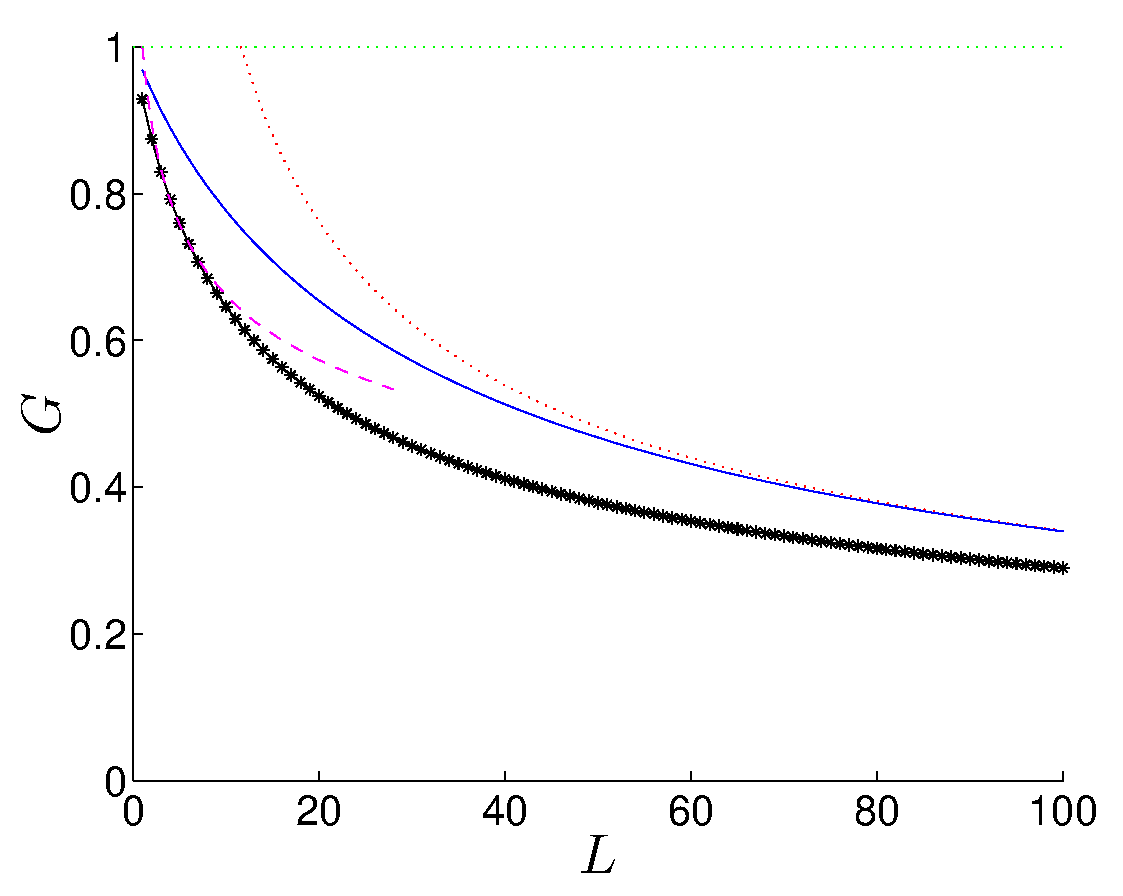
\includegraphics[clip,width=4cm]{G_versus_L}
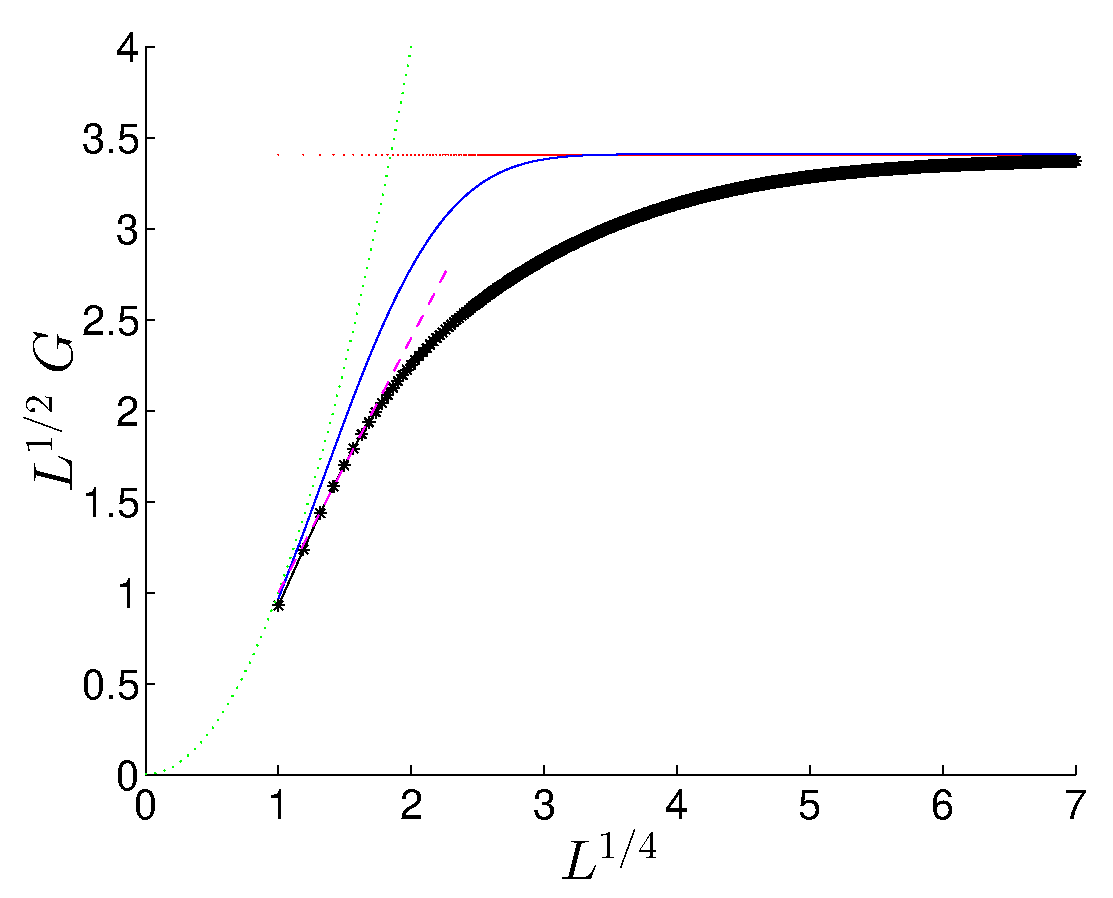
\includegraphics[clip,width=4cm]{GsqrtL_sqrtL}

\caption{
The heat conductance $G$ as a function of $L$ is calculated using \Eq{e5} with \Eq{e5}.
For the black solid line with symbols we use $\gamma(k)$ that is based on the numerical
results that have been obtained for a logbox disorder as in \Fig{f2}a with ${\sigma=1}$.  
For the blue solid line we use the Debye approximation for the density 
of states, and extrapolate the initial $\gamma\propto k^2$ dependence up to the cutoff $k=\pi$.  
%
On the right panel we plot $\sqrt{L}G$ as a function of $L^{1/4}$ 
in order to highlight the ${\alpha=1/2}$ (dotted red) and the ${\alpha=1/4}$ (dashed red)
asymptotic dependence for long and short samples respectively. 
The green dotted line is $G=1$. }

\label{f4}
\end{figure}





%%%%%%%%%%%%%%%%%%%%%%%%%%%%%%%%%%%%%%%%%%%%%%%%%%%%%%%%%%
\sect{Heat conductance}
%
Following  \cite{D08,D01,DL08} the expression for the rate of heat flow from 
a lead that has temperature $T_H$ to a lead that has temperature $T_C$ is 
% 
\beq
\dot{Q} \ = \ 
\frac{T_H{-}T_C}{2} \int_{0}^{\infty} \frac{d\omega}{\pi} \ \mathcal{T}(\omega) 
\ \equiv \ G \, (T_H{-}T_C) \ \ 
\label{qg}
\eeq
%
Here $\mathcal{T}(\omega)$ is a complicated expression that reflects 
the transmission of the sample.  
If we were dealing with incoherent or non-linear transport \cite{dubi}, 
it would be possible to justify the Ohmic expression ${\mathcal{T}(\omega)=\ell/L}$, 
where $\ell$ is the inelastic mean free path. 
But we are dealing with an isolated harmonic chain, 
therefore ${\mathcal{T}(\omega)}$ is determined by 
the couplings of the eigenmodes to the heat reservoirs
at the left and right leads. 
In analogy to mesoscopics studies \cite{D08,D01} one can argue that
%
\beq
\mathcal{T}(\omega) \ \ \approx \ \ g(\omega) \ \mathcal{T}^{(0)}(\omega)
\eeq
%
where $\mathcal{T}^{(0)}(\omega)$ refers to a non-disordered sample, 
and $g(\omega)$ is the disordered averaged transmission. 
For ``fixed boundary conditions" ${\mathcal{T}^{(0)}(\omega)\sim \eta_0^2\omega^2}$,
where the damping rate $\eta_0$ characterizes the contact point.
In contrast, for ``free boundary condition" one obtains ${\mathcal{T}^{(0)}(\omega)\approx 1}$, 
which is the most optimal possibility. In the latter case  
%
\be{17}
G \ \ = \ \ \frac{c}{2} \int_0^{\pi} \frac{d k}{\pi} \ g(\omega_k) 
\eeq
%
The standard approach is to use two {\em incompatible} approximations:
On the one hand one use the asymptotic estimate ${g(\omega) \sim \eexp{-(1/2)\gamma(\omega) L}}$ 
which holds for {\em long} samples for which $\gamma L\gg 1$. 
On the other hand one extends the upper limit of the integration to infinity, 
arguing that the major contribution to the integral comes from small $\omega$ values.
% 
In the absence of pinning $\gamma(\omega)\propto\omega^2$, hence by rescaling 
of the dummy integration variable it follows that the result of the integral 
is precisely $\propto 1/\sqrt{L}$. 
%
We shall discuss in the next paragraph the limitations of this prediction. 
Going on with the same logic we can ask what happens in the presence of 
a weak pinning potential. Using a saddle-point estimate 
we get $G \sim  \frac{1}{\sqrt{L}} \ \exp\left[ -(1/2) \gamma_0 L \right]$, 
where $\gamma_0$ is the minimal value of $\gamma(\omega)$. 
From \Eq{FGRw} with \Eq{FGRv} we deduce $\gamma_{0} \propto b^{-\eta}$, with $\eta=7/2$.
This explains the leading exponential dependence on the length 
that has been observed in \cite{BZFK13}. 
However the above calculation fails in explaining the 
sub-leading $L$ dependence that survives in the absence of pinning.
Namely it has been observed that instead of $1/L^{\alpha}$ with $\alpha=1/2$
the numerical results are characterized by the super-optimal value ${\alpha \approx 1/4}$.  


%%%%%%%%%%%%%%%%%%%%%%%%%%%%%%%%%%%%%%%%%%%%%%%%%%%%%%%%%%
\sect{Beyond the asymptotic estimate}
%
We now focus on the $L$ dependence the survives in the absence of a pinning potential.
As already note that deviation from the $1/\sqrt{L}$ law is related to two incompatible 
approximations regarding the~$\gamma$ dependence of~$g$ 
and the upper limit of of the integration in \Eq{e17}.    
We can of course do better by using the analytical expression \Eq{e14}.
For the density of states we can use either numerical results 
or optionally we can use the Debye approximation. The latter 
may affect the results {\em quantitatively} but not qualitatively.
Within the framework of the Debye approximation we assume 
idealized dependence $\gamma(\omega_k) \propto \sigma_{\perp}^2 k^2$ 
in accordance with \Eq{FGRw}, up to the cutoff at $k=\pi$.
%
The result of the calculation is presented in \Fig{f4}.  
On the right panel there we plot $\sqrt{L}G$ as a function of $L^{1/4}$ 
in order to highlight the ${\alpha=1/2}$ and the ${\alpha=1/4}$ 
asymptotic dependence for long and short samples respectively. 
Note that in the latter case, as in \cite{BZFK13},  
a small offset has been included in the fitting procedure.
We do not think that the ${\alpha=1/4}$ dependence is ``fundamental". 
The important message here is that a straightforward application 
of an analytical approach can explain the failure of the $1/\sqrt{L}$ law. 
We also see that the numerical prefactor of the $1/L^{\alpha}$ dependence 
is sensitive to the line-shape of the large~$k$ cutoff, 
hence it is not the same for the numerical spectrum and for its Debye approximation. 
\\

%%%%%%%%%%%%%%%%%%%%%%%%%%%%%%%%%%%%%%%%%%%%%%%%%%%%%%%%%%
\sect{Conclusions} 
%
We have considered in this work the problem 
of heat conduction of quasi one-dimensional ($b\gg1$) 
as well as single channel harmonic chains; 
addressing the effects of both glassy disorder (couplings) and pinning (diagonal disorder).
We were able to provide a theory for the asymptotic exponential 
length ($L$) and bandwidth ($b$) dependence; as well as for the 
algebraic $L$~dependence in the absence of a pinning potential. 
A major observation along the way was the duality between 
glassy disorder and weak Anderson disorder. That helped 
us to figure out what is the effective hopping~$w_0$, 
hence establishing a relation to percolation theory.
It also helped us to go beyond the naive Born approximation
that cannot be justified for glassy disorder, 
and to identify a (dual) Lifshitz anomaly in 
the $\omega$ dependence of the transmission. 
Finally, we have established that known results from 
one-parameter scaling theory can be utilized in order 
to derive the non-asymptotic $L$ dependence of the heat conductance. \\  
     

%%%%%%%%%%%%%%%%%%%%%%%%%%%%%%%%%%%%%%%%%%%%%%%%%%%%%%%%%%%%%%%%
%%%%%%%%%%%%%%%%%%%%%%%%%%%%%%%%%%%%%%%%%%%%%%%%%%%%%%%%%%%%%%%%

\noindent
{\bf Acknowledgements.-- }
This research has been supported by  by the Israel Science Foundation (grant No. 29/11).


%%%%%%%%%%%%%%%%%%%%%%%%%%%%%%%%%%%%%%%%%%%%%%%%%%%%%%%%%%%%%%%%
%%%%%%%%%%%%%%%%%%%%%%%%%%%%%%%%%%%%%%%%%%%%%%%%%%%%%%%%%%%%%%%%

\begin{thebibliography}{99}

\bibitem{LLP03} 
S. Lepri, R. Livi, \& A. Politi, 
%{\em Thermal conduction in classical low-dimensional lattices},
Phys. Rep. {\bf 377}, 1 (2003).

\bibitem{D08} 
A. Dhar, 
%{\em Heat transport in low-dimensional systems}, 
Adv. Phys. {\bf 57}, 457 (2008).

\bibitem{LRWZHL12} 
N. Li, J. Ren, L. Wang, G. Zhang, P. H\"anggi, and B. Li, 
%{\em Colloquium: Phononics: Manipulating heat flow with electronic analogs and beyond}, 
Rev. Mod. Phys. \textbf{84}, 1045 (2012).


\bibitem{COGMZ08}
C.W. Chang, D. Okawa, H. Garcia, A. Majumdar,  A. Zettl, 
%{\em Breakdown of Fourier’s Law in Nanotube Thermal Conductors}, 
Phys. Rev. Lett, {\bf 101}, 075903 (2008).

\bibitem{NGPB09} 
D.L. Nika, S. Ghosh, E. P. Pokatilov, and A. A. Balandin, 
% {\em Lattice thermal conductivity of graphene flakes: Comparison with bulk graphite}, 
Appl. Phys. Lett. {\bf 94}, 203103 (2009).


\bibitem{ZL10} 
G. Zhang, B. Li,
% {\em Impacts of Doping On Thermal and Thermoelectric Properties of Nan-Materials"},  
NanoScale {\bf 2}, 1058 (2010).

\bibitem{K1} 
H. Li, T. Kottos, B. Shapiro, 
% Thermal transport in phononic Cayley-tree networks
Phys. Rev. E  91, 042125 (2015).

\bibitem{K2} 
M. Schmidt, T. Kottos, B. Shapiro,
% Random-matrix-theory approach to mesoscopic fluctuations of heat current
Phys. Rev. E  88, 022126 (2013).

\bibitem{D01}
A. Dhar, 
% {\em Heat Conduction in the Disordered Harmonic Chain Revisited}, 
Phys. Rev. Lett. {\bf 86}, 5882 (2001).

\bibitem{LXXZL12} 
S. Liu, X. Xu, R. Xie, G. Zhang, B. Li, 
% Anomalous Heat Conduction and Anomalous Diffusion in Low Dimensional Nanoscale Systems
Euro. Phys. J. B 85, 337 (2012).
% arXiv:1205.3065v2 [cond-mat.stat-mech] (2012).

\bibitem{DL08} 
A. Dhar, J.L. Lebowitz, 
Phys. Rev. Lett. {\bf 100}, 134301 (2008).

\bibitem{LD05} 
L. W. Lee, A. Dhar, 
Phys. Rev. Lett. {\bf 95}, 094302 (2005).

\bibitem{RD08} 
D. Roy, A. Dhar, 
Phys. Rev. E {\bf 78}, 051112 (2008).

\bibitem{LZH01} 
B. Li, H. Zhao, B. Hu, 
Phys. Rev. Lett. {\bf 86}, 63 (2001).

\bibitem{KCRDLS10a}
A. Kundu, A. Chaudhuri, D. Roy, A. Dhar, J.L. Lebowitz, H. Spohn,
Europhys. Lett. {\bf 90}, 40001 (2010).

\bibitem{KCRDLS10b}
A. Chaudhuri, A. Kundu, D. Roy, A. Dhar, J.L. Lebowitz, H. Spohn,
% Heat transport and phonon localization in mass-disordered harmonic crystals
Phys. Rev. B {\bf 81}, 064301 (2010).

\bibitem{BZFK13}
J.D. Bodyfelt, M. C. Zheng, R. Fleischmann, T. Kottos, 
Phys. Rev. E {\bf 87}, 020101(R) (2013)

\bibitem{DG84}
B. Derrida and E. Gardner, 
J. Physique {\bf 45}, 1283 (1984). 

\bibitem{Abrikosov}
A.A. Abrikosov, 
% The paradox with the static conductivity of a one-dimensional metal,
Solid State Communications {\bf 37}, 997 (1981)

\bibitem{Shapiro}
B. Shapiro, 
%Probability distributions in the scaling theory of localization
Phys. Rev. B 34, R4394 (1986)
%http://journals.aps.org/prb/abstract/10.1103/PhysRevB.34.4394


\bibitem{Izrailev}
F.M. Izrailev, A.A. Krokhin, N.M. Makarov,
%Anomalous localization in low-dimensional systems with correlated disorder
Physics Reports 512, 125 (2012).
% http://www.sciencedirect.com/science/article/pii/S0370157311002936

\bibitem{dubi}
Y. Dubi, M. Di Ventra,
%Fourier’s law: Insight from a simple derivation
Phys. Rev. E 79, 042101 (2009).
% http://journals.aps.org/pre/abstract/10.1103/PhysRevE.79.042101

\bibitem[a]{rmrkA}
Given an eigenstate $\psi$ we define $p_n=|\psi_n|^2$.
The normalization is such that $\sum p_n=1$. 
The participation number PN$=[\sum p_n^2]^{-1}$ 
is a measure for the number of sites that are occupied 
by the eigenstate.

\end{thebibliography}



%%%%%%%%%%%%%%%%%%%%%%%%%%%%%%%%%%%%%%%%%%%%%%%%%%%%%%%%%%%%%%%%
%%%%%%%%%%%%%%%%%%%%%%%%%%%%%%%%%%%%%%%%%%%%%%%%%%%%%%%%%%%%%%%%
\clearpage
\end{document}



%%%%%%%%%%%%%%%%%%%%%%%%%%%%%%%%%%%%%%%%%%%%%%%%%%%%%%%%%%%%%%%%
%%%%%%%%%%%%%%%%%%%%%%%%%%%%%%%%%%%%%%%%%%%%%%%%%%%%%%%%%%%%%%%%
%%%%%%%%%%%%%%%%%%%%%%%%%%%%%%%%%%%%%%%%%%%%%%%%%%%%%%%%%%%%%%%%
%%%%%%%%%%%%%%%%%%%%%%%%%%%%%%%%%%%%%%%%%%%%%%%%%%%%%%%%%%%%%%%%



% optimal g
%%%%%%%%%%%%%%%%%%%%%%%%%%%%%%%%%%%%%%%%%%%%%%%%%%%%%%%%%%%%
\begin{figure}
\includegraphics[clip,width=6cm]{g_hopping}
	
\caption{The average conductance as a function of the hopping rate $w_0$ within the leads. \\
We assume conservative log-box disorder with $\sigma=10$ and $k=0.0056\pi$.}

\label{g_hopping} \label{f12}
\end{figure}






